\documentclass[letterpaper, landscape]{exam}
\usepackage{2in1, lscape} 
\printanswers

\usepackage{units} 
\usepackage[fleqn]{amsmath}
\usepackage{float}
\usepackage{mdwlist}
\usepackage{booktabs}
\usepackage{caption}
\usepackage{fullpage}
\usepackage{enumerate}
\usepackage{graphicx}
\usepackage[justification=justified]{caption}

\setcounter{tocdepth}{1}
\everymath{\displaystyle}

\author{}
\date{\today}
\title{Calculus I \\ Week Fifteen}

\begin{document}

  \maketitle
  \tableofcontents
  \section{Homework 13} % (fold)
  \label{sec:Homework 13}

  When finding the second derivative using implicit differentiation, make sure to go back and plug
  in the first derivative in the answer. Answer key didn't do this.
  
  \section{Section 4.1} % (fold)
  
  \subsection{Minimum/Maximum} % (fold)

  \begin{itemize}
    \item absolute min/max is smallest/largest $f(x)$ in the domain
    \item Local max at $x = a$ means for all $b$ in some open interval around $a$, $f(a) > f(b)$
  \end{itemize}

  \subsection{Extreme Value Theorem} % (fold)
  
  If $f$ is continuous on closed interval $[a, b]$ then it has a maximum and minimum in that
  interval.

  Continuous and closed matter because you might have a vertical asymptote or undefined value where
  \[
    \lim_{x \to a} f(a) = L
  \]

  but $f(a)$ isn't defined so there is no maximum
  
  \subsection{Fermat's Theorem} % (fold)
  
  two ways of saying it:
  \begin{itemize*}
    \item If $f$ has a local min/max at $c$ and $f'(c)$ exists, then $f'(c) = 0$ 
    \item If $f$ has a local min/max at $c$ then $f'(c) = 0$ or $f'(c)$ doesn't exist.
    \item If $f$ has a local min/max at $c$ then $c$ is a critical number
  \end{itemize*}

  Values where $f'(c) = 0$ or $f'(c)$ is not defined are {\em critical numbers}.

  \begin{itemize*}
    \item Draw local max with $f'$ exists and $f'$ doesn't exist.
    \item Draw $f(x) = x^3$ where $f'(0) = 0$ and there is no min/max at $x = 0$
    \item Draw $f(x) = \frac{1}{x}$ where $f'(0)$ doesn't exist and there is no min/max at $x = 0$
  \end{itemize*}

  \subsection{Absolute Maximums} % (fold)
  
  To find absolute min/max for a continuous function on a closed interval, 

  \begin{itemize*}
    \item find all the critical numbers
    \item evaluate $f$ at all the critical numbers and endpoints
    \item largest value is max and smallest value is min
  \end{itemize*}

  \subsection{Examples} % (fold)

  \begin{description}

    \item[49] $f(x) = 2x^3 - 3x^2 -12x + 1$; $[-2, 3]$
      \begin{solution}
        \begin{tabular}[H]{rr}
          \toprule
          $x$ & $f(x)$ \\
          \midrule
          $-2$  & $-3$ \\
          $-1$  & $8$ \\
          $2$   & $-19$ \\
          $3$   & $-8$ \\
          \bottomrule
        \end{tabular}
      \end{solution}

      \begin{figure}[H]
        \centering
        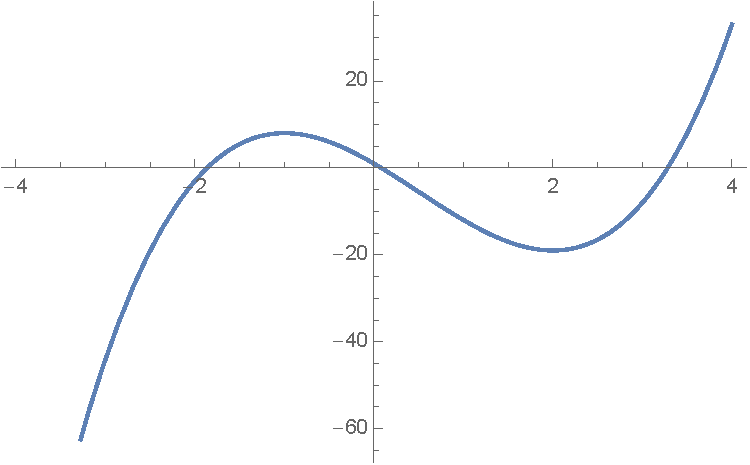
\includegraphics[scale = 0.6]{ex41_49.pdf}
        \caption{Exercise 49}
        \label{fig:ex41_49}
      \end{figure}

    \item[54]
      $f(x) = \frac{x^2 - 4}{x^2 + 4}$ $[-4, 4]$

      \begin{solution}
        $f'(x) = \frac{16x}{\left(x^2 + 4\right)^2}$

        \begin{tabular}[H]{rr}
          \toprule
          $x$  & $f(x)$ \\
          \midrule
          $-4$ & $\frac{3}{5}$ \\
          $0$  & $-1$ \\
          $4$  & $\frac{3}{5}$ \\
          \bottomrule
        \end{tabular}

        \begin{figure}[H]
          \centering
          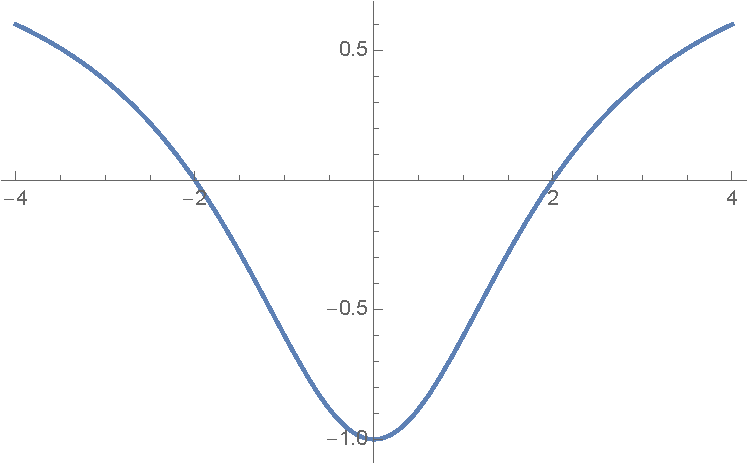
\includegraphics[scale = 0.6]{ex41_54.pdf}
        \caption{Exercise 54}
        \label{fig:ex41_54}
        \end{figure}
      \end{solution}

  \end{description}

\end{document}

